\documentclass[a4paper,12pt]{article} % тип документа

%  Русский язык
\usepackage[T2A]{fontenc}			% кодировка
\usepackage[utf8]{inputenc}			% кодировка исходного текста
\usepackage[english,russian]{babel}	% локализация и переносы

\usepackage{graphicx}               % импорт изображений
\usepackage{wrapfig}                % обтекаемые изображения
\graphicspath{{pictures/}}          % обращение к подкаталогу с изображениями
\usepackage[14pt]{extsizes}         % для того чтобы задать нестандартный 14-ый размер шрифта
\usepackage{amsfonts}               % буквы с двойными штрихами
\usepackage[warn]{mathtext}         % русский язык в формулах
\usepackage{indentfirst}            % indent first
\usepackage[margin = 25mm]{geometry}% отступы полей
\usepackage{amsmath}                % можно выводить фигурные скобочки -- делать системы уравнений
\usepackage[table,xcdraw]{xcolor}   % таблицы
\usepackage{amsmath,amsfonts,amssymb,amsthm,mathtools} % Математика
\usepackage{wasysym}                % ???
\usepackage{upgreek}                % ???  
\usepackage{caption}
\captionsetup{labelsep=period}
\usepackage{gensymb} % degree symbol
\usepackage{mathrsfs}
\usepackage{multirow}

\begin{document}
	\begin{center}
		
		\textbf{НАЦИОНАЛЬНЫЙ ИССЛЕДОВАТЕЛЬСКИЙ УНИВЕРСИТЕТ \\ <<МОСКОВСКИЙ ФИЗИКО-ТЕХНИЧЕСКИЙ ИНСТИТУТ>>}
		\vspace{13ex}
		
		\textbf{Лабораторная работа 3.4.5 \\ <<Петля гистерезиса (динамический метод)>> }
		\vspace{60ex}
		
		\normalsize{Овсянников Михаил Александрович \\ студент группы Б01-001\\ 2 курс ФРКТ\\}
	\end{center}
	
	\vfill 
	
	\begin{center}
		г. Долгопрудный\\ 
		2021 г.
	\end{center}
	
	\thispagestyle{empty} % выключаем отображение номера для этой страницы
	
	\newpage
	
	\textbf{Цель работы:} изучение петель гистерезиса ферромагнитных материалов с помощью осциллографа.
	
	\vspace{7mm}
	\textbf{Оборудование:} автотрансформатор, понижающий трансформатор, амперметр и вольтметр (мультиметры), резистор, делитель напряжения, интегрирующая
	цепочка, электронный осциллогра, тороидальные образцы с двумя обмотками.
	
	
	\section*{Теоретические сведения}
	
	\begin{wrapfigure}{l}{0.6\textwidth}
		\vspace{-20pt}
		\begin{center}
			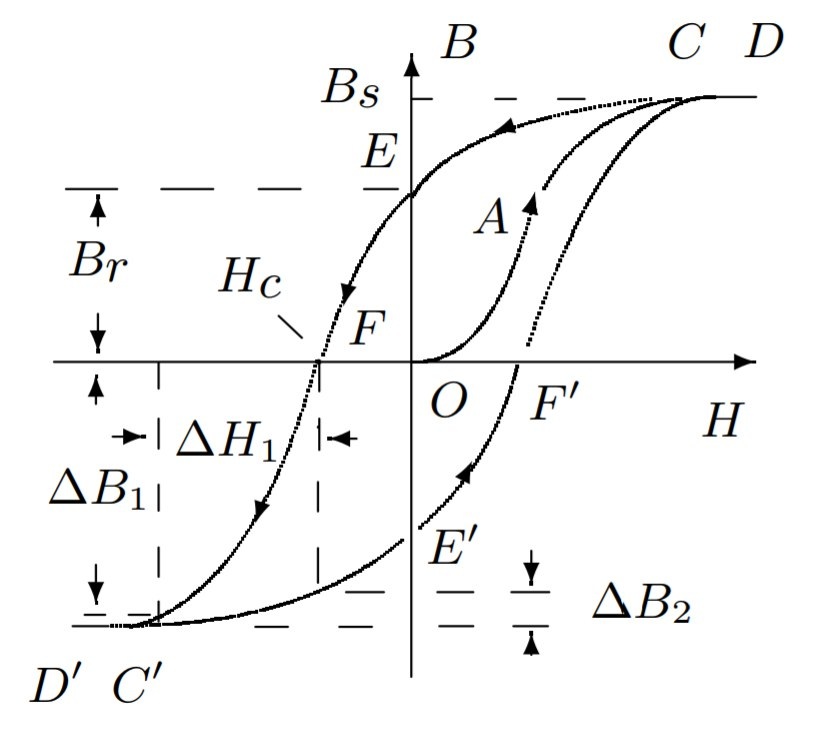
\includegraphics[width=0.7\linewidth]{Pictures/Loop.jpeg}
		\end{center}
		\vspace{-10pt}
		\caption{Петля гистерезиса ферромагнетика}
	\end{wrapfigure}
	
	Магнитная индукция $\vec{B}$ и напряженность магнитного поля
	$\vec{H}$ в ферромагнитном материале неоднозначно связаны
	между собой: индукция зависит не только от напряженности, но
	и от предыстории образца. Связь между индукцией
	и напряженностью поля типичного ферромагнетика иллюстрирует рис. 1. Если
	к размагниченному образцу начинают прикладывать магнитное поле, то его намагничивание следует кривой $ OACD $, выходящей
	из начала
	координат. Эту кривую называют основной кривой намагничивания.
	
	
	Индукция $\vec{B}$ в образце состоит из индукции, связанной с намагничивающим полем
	$\vec{B}$, и индукции, создаваемой самим намагниченным
	образцом.
	В системе СИ эта связь имеет вид
	
	$$\vec{B} = \mu_{0}(\vec{H}+\vec{I}),$$
	
\noindent	где $\vec{I}$- намагниченность - магнитный момент единичного объема образца, а $\mu_{0}$ - магнитная постоянная.

\newpage
\section*{Экспериментальная установка.}
Схема экспериментальной установки показана на рис. 2.

Действующее значение переменного тока в обмотке $N_0$ измеряется амперметром А (мультиметром GDM). Последовательно с амперметром включено сопротивление $R_{0}$, напряжение с которого подается на вход X электронного осциллографа (ЭО). Это напряжение пропорционально току в обмотке $N_{0}$, а следовательно и напряженности $H$ магнитного поля в образце.

Для измерения магнитной индукции $B$ с измерительной обмотки $N_{И}$ на вход интегрирующей $RC$-цепочки подается напряжение $U_{\text{И}}$, пропорциональное производной $\dot{B}$, а с выхода снимается напряжение $U_{C}$($U_{\text{ВЫХ}}$), пропорциональное величине $B$ , и подается на вход Y осциллограа.
Замкнутая кривая, возникающая на экране, воспроизводит в некотором масштабе (различном для осей X и Y ) петлю гистерезиса. Чтобы придать этой кривой количественный смысл, необходимо установить масштабы изображения, т.е. провести калибровку каналов X и Y ЭО. Для этого, во-первых, надо узнать, каким напряжениям (или токам) соответствуют амплитуды сигналов, видимых на экране, и во-вторых,  каким значениям $B$ и $H$ соответствуют эти напряжения (или токи).

\begin{figure}[h!]
	\centering
	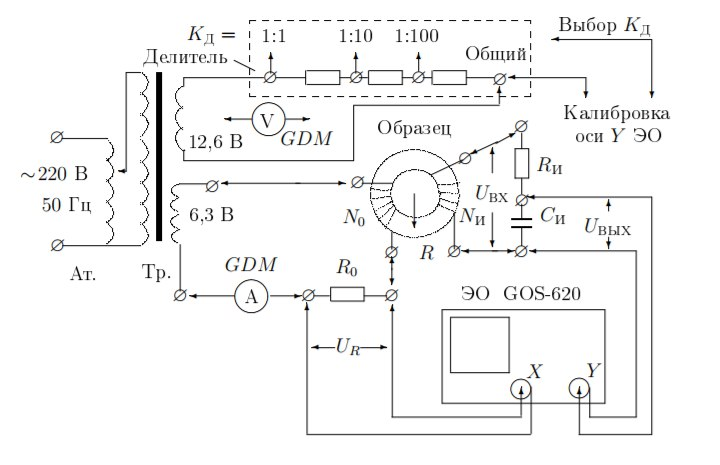
\includegraphics[width=\linewidth]{Pictures/Scheme.jpeg}
	\caption{Схема установки для исследования намагничивания образцов}
\end{figure}

\newpage
Выпишем основные формулы, которые понадобятся в данной работе.

Поле $H$:  $H = \dfrac{IN_0}{2\pi R}$,   $R$ - радиус тороидального соленоида (образца)

\vspace{7mm}
Поле $B$:  $B = \dfrac{RCU}{SN_u}$,      $R$ и $C$ - параметры $RC$-цепи. $RC = 0,4$ с.

\section*{Ход работы}

Проведем серию из трех экспериментов - для трех образцов: феррита, пермаллоя и кремнистого железа.

Сначала зафиксируем параметры конкретного образца. Затем будем находить значения тока $I_{\text{пр}}$ и напряжения $U_{\text{пр}}$, при которых наблюдается предельная петля гистерезиса. Далее - для первых двух образцов рассчитаем поле $H$ и поле $B$ по параметрам их параметрам. И, наконец, найдем магнитную проницаемость $\mu$ образца при данном токе и напряжении. В каждом эксперименте будем сводить все в таблицу.

\vspace{8mm}
\textbf{{\large Феррит (Fe)}}

\begin{figure}[h!]
	\centering
	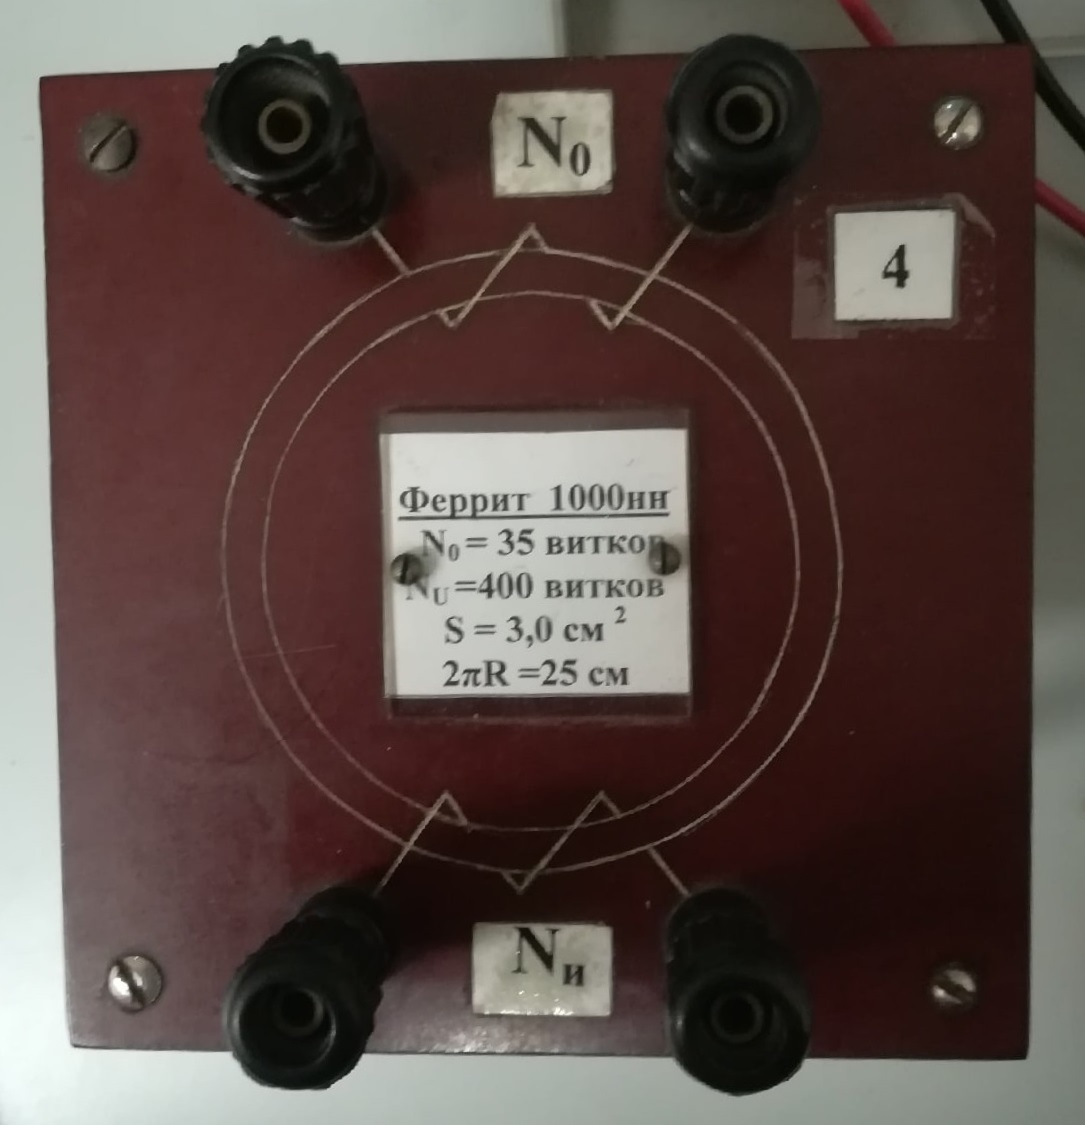
\includegraphics[scale=0.47]{Pictures/ФЕРРИТ.jpg}
	\caption{Феррит}
\end{figure}

Параметры образца:

$N_0 = 35;$

$N_u = 400;$

$S = 3,0$ см$^2$;

$2\pi R = 25$ см.

\vspace{7mm}
Предельные значения тока и напряжения:

$I_{\text{пр}} = 132,37$ мА, $U_{\text{пр}} = 36,62$ мВ.

\begin{figure}[h!]
	\centering
	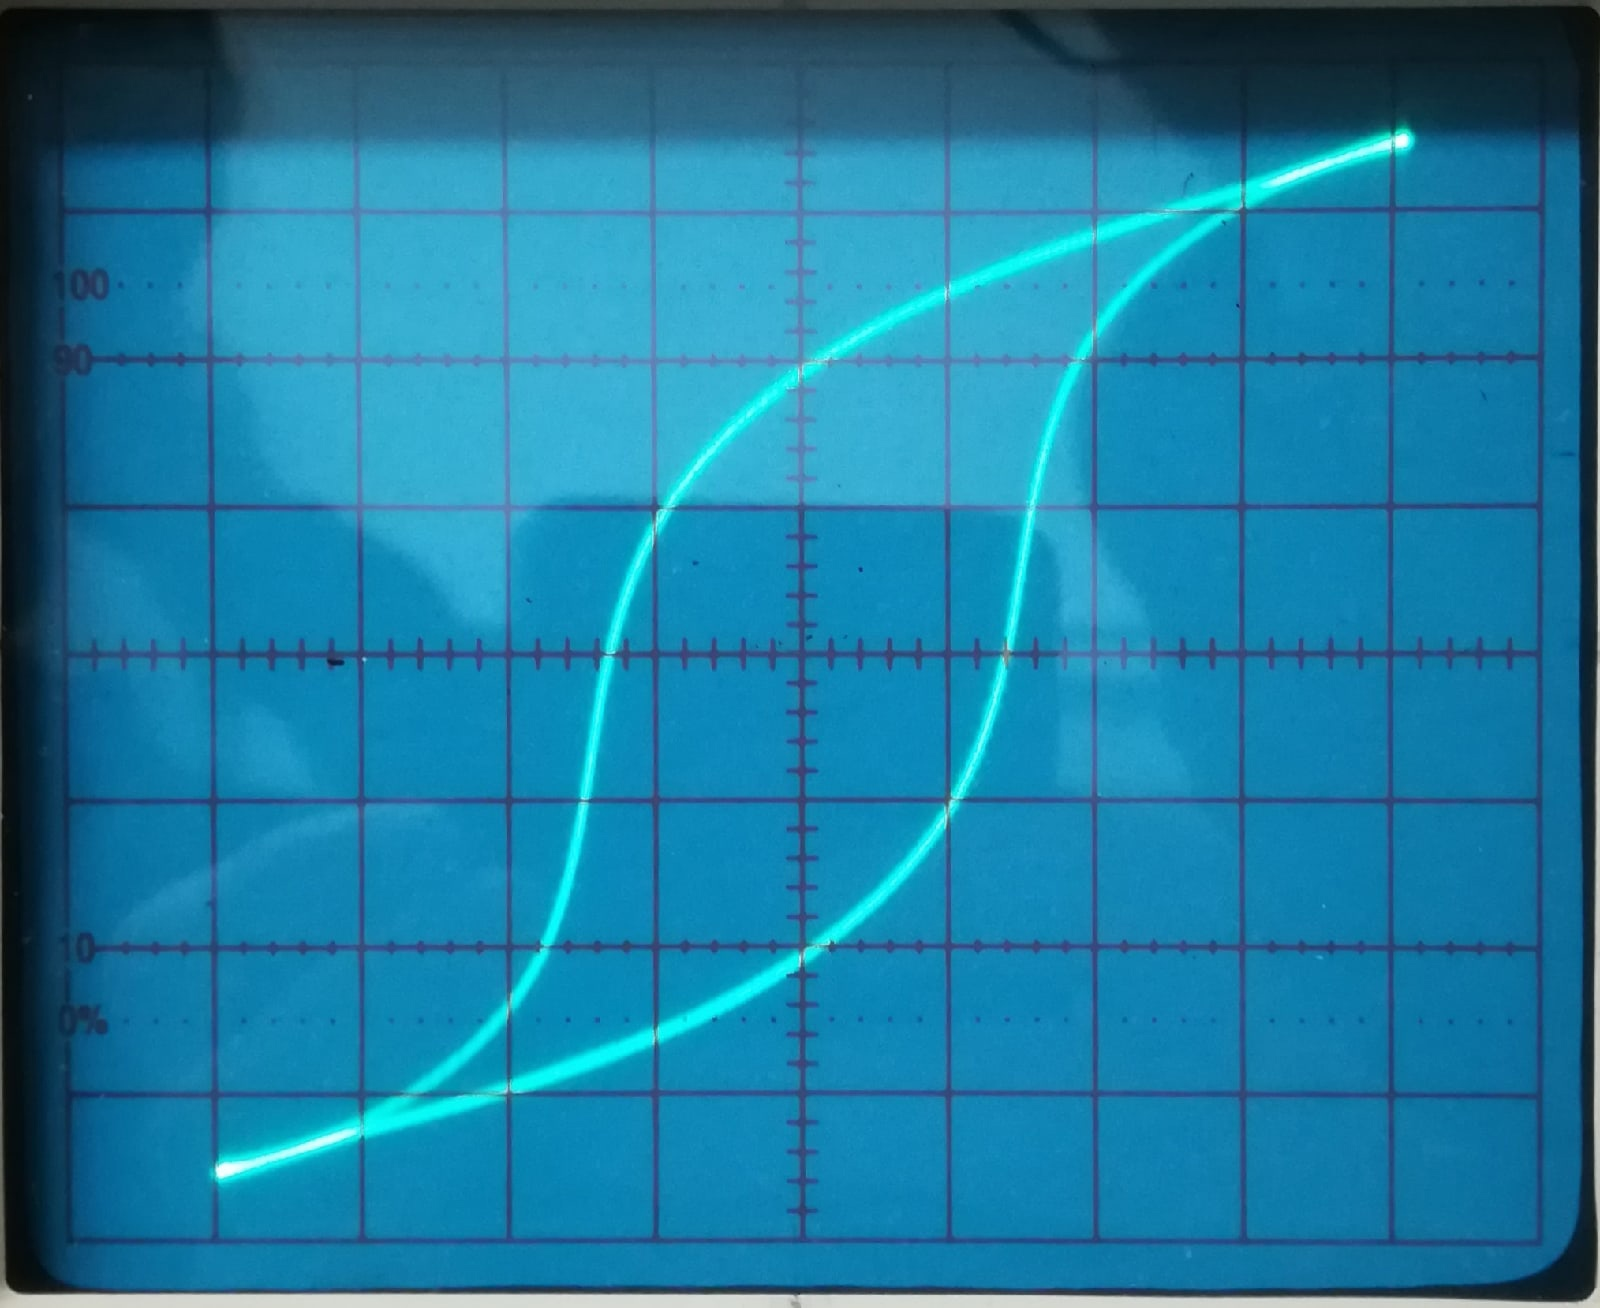
\includegraphics[scale=0.27]{Pictures/ФЕРРИТ_ПЕТЛЯ.jpg}
	\caption{Петля гистерезиса. Феррит}
\end{figure}

\newpage
Сведем все данные в таблицу.


\begin{table}[h!]
	\centering
	\begin{tabular}{|l|l|l|l|l|l|l|}
		\hline
		\multicolumn{1}{|c|}{$I_{\text{эф}}$, мА} & \multicolumn{1}{c|}{$I_{\text{эф}} \cdot \sqrt{2}$, мА} & \multicolumn{1}{c|}{$H$, $\frac{\text{А}}{\text{м}}$} & \multicolumn{1}{c|}{$U_{\text{эф}}$, мВ} & \multicolumn{1}{c|}{$U_{\text{эф}} \cdot \sqrt{2}$, мВ} & \multicolumn{1}{c|}{$B$, Тл} & \multicolumn{1}{c|}{$\mu = \dfrac{B}{\mu_0 H}$} \\ \hline
		24,1                                      & 34,01                                                   & 4,76                                                  & 3,0                                      & 4,24                                                    & 0,014                        & 2363,46                                         \\ \hline
		27,3                                      & 38,65                                                   & 5,41                                                  & 4,6                                      & 6,51                                                    & 0,022                        & 3189,04                                         \\ \hline
		29,9                                      & 42,31                                                   & 5,92                                                  & 6,1                                      & 8,63                                                    & 0,029                        & 3862,86                                         \\ \hline
		32,1                                      & 45,34                                                   & 6,35                                                  & 7,6                                      & 10,75                                                   & 0,036                        & 4491,50                                         \\ \hline
		34,3                                      & 48,55                                                   & 6,80                                                  & 9,1                                      & 12,87                                                   & 0,043                        & 5022,37                                         \\ \hline
		36,4                                      & 51,42                                                   & 7,20                                                  & 10,6                                     & 14,99                                                   & 0,050                        & 5523,61                                         \\ \hline
		38,6                                      & 54,59                                                   & 7,64                                                  & 12,0                                     & 16,97                                                   & 0,057                        & 5890,27                                         \\ \hline
		41,3                                      & 58,44                                                   & 8,18                                                  & 13,7                                     & 19,37                                                   & 0,065                        & 6282,05                                         \\ \hline
		44,2                                      & 62,54                                                   & 8,76                                                  & 15,0                                     & 21,21                                                   & 0,071                        & 6427,08                                         \\ \hline
		50,9                                      & 71,94                                                   & 10,07                                                 & 17,5                                     & 24,75                                                   & 0,082                        & 6518,05                                         \\ \hline
		57,8                                      & 81,74                                                   & 11,44                                                 & 19,0                                     & 26,87                                                   & 0,090                         & 6228,26                                         \\ \hline
		63,9                                      & 90,30                                                   & 12,64                                                 & 20,5                                     & 28,99                                                   & 0,097                        & 6083,23                                         \\ \hline
		70,1                                      & 99,14                                                   & 13,88                                                 & 22,0                                     & 31,11                                                   & 0,104                        & 5946,29                                         \\ \hline
		78,4                                      & 110,87                                                  & 15,52                                                 & 23,5                                     & 33,23                                                   & 0,111                        & 5679,28                                         \\ \hline
		88,2                                     & 124,69                                                  & 17,46                                                 & 25,0                                     & 35,36                                                   & 0,118                        & 5372,30                                         \\ \hline
		99,1                                      & 140,15                                                  & 19,62                                                 & 26,5                                     & 37,48                                                   & 0,125                        & 5066,56                                         \\ \hline
		111,7                                     & 157,97                                                  & 22,12                                                 & 28,0                                     & 39,60                                                    & 0,132                        & 4749,48                                         \\ \hline
		126,3                                     & 178,62                                                  & 25,01                                                 & 29,5                                     & 41,72                                                   & 0,139                        & 4425,47                                         \\ \hline
		144,2                                     & 203,86                                                  & 28,54                                                 & 31,0                                     & 43,84                                                   & 0,146                        & 4074,63                                         \\ \hline
		164,3                                     & 232,36                                                  & 32,53                                                 & 32,5                                     & 45,96                                                   & 0,153                        & 3747,89                                         \\ \hline
	\end{tabular}
	\caption{Феррит}
\end{table}

\newpage
Теперь построим графики.

\begin{figure}[h!]
	\centering
	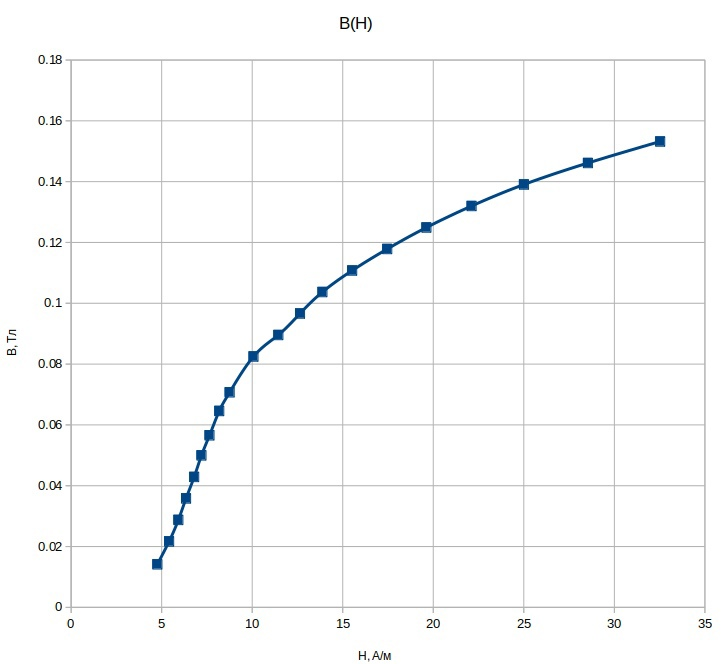
\includegraphics[scale=0.43]{Pictures/ФЕРРИТ_B(H).jpg}
	\caption{Феррит. $B(H)$}
\end{figure}

\begin{figure}[h!]
	\centering
	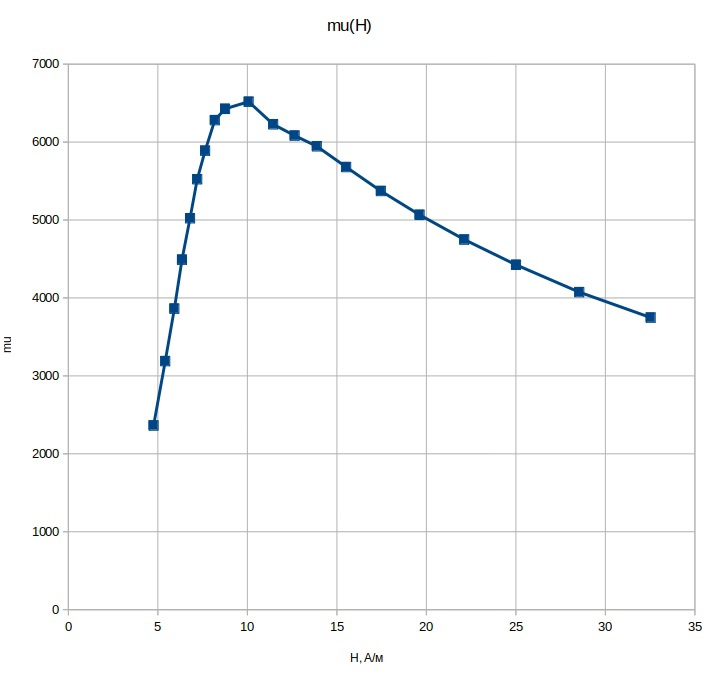
\includegraphics[scale=0.43]{Pictures/ФЕРРИТ_mu(H).jpg}
	\caption{Феррит. $\mu (H)$}
\end{figure}



\newpage
\textbf{{\large Пермаллой (Fe-Ni)}}
\begin{figure}[h!]
	\centering
	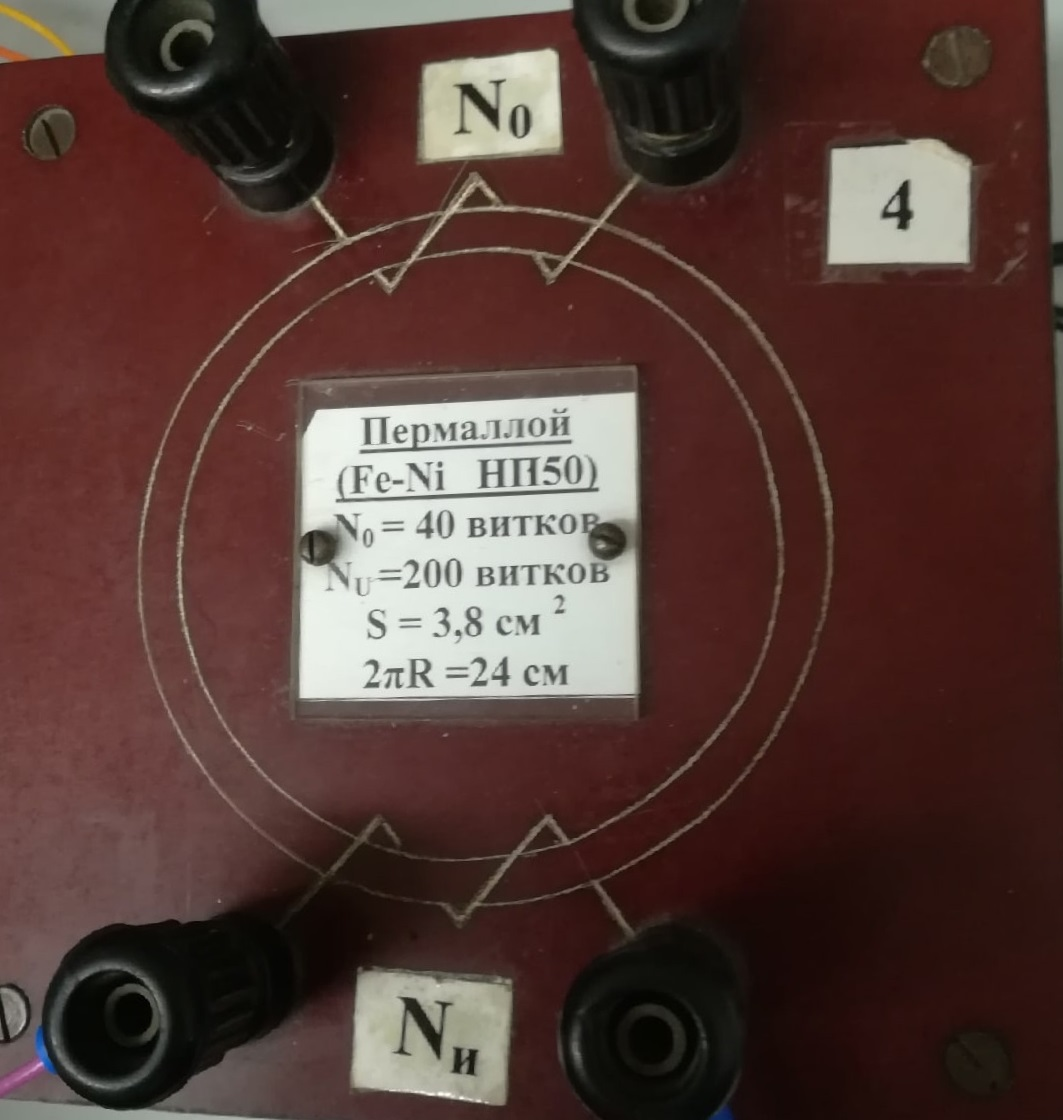
\includegraphics[scale=0.6]{Pictures/ПЕРМАЛЛОЙ.jpg}
	\caption{Пермаллой}
\end{figure}

Параметры образца:

$N_0 = 40;$

$N_u = 200;$

$S = 3,8$ см$^2$;

$2\pi R = 24$ см.

\vspace{7mm}
Предельные значения тока и напряжения:

$I_{\text{пр}} = 233,54$ мА, $U_{\text{пр}} = 169,28$ мВ.
\newpage
\begin{figure}[h!]
	\centering
	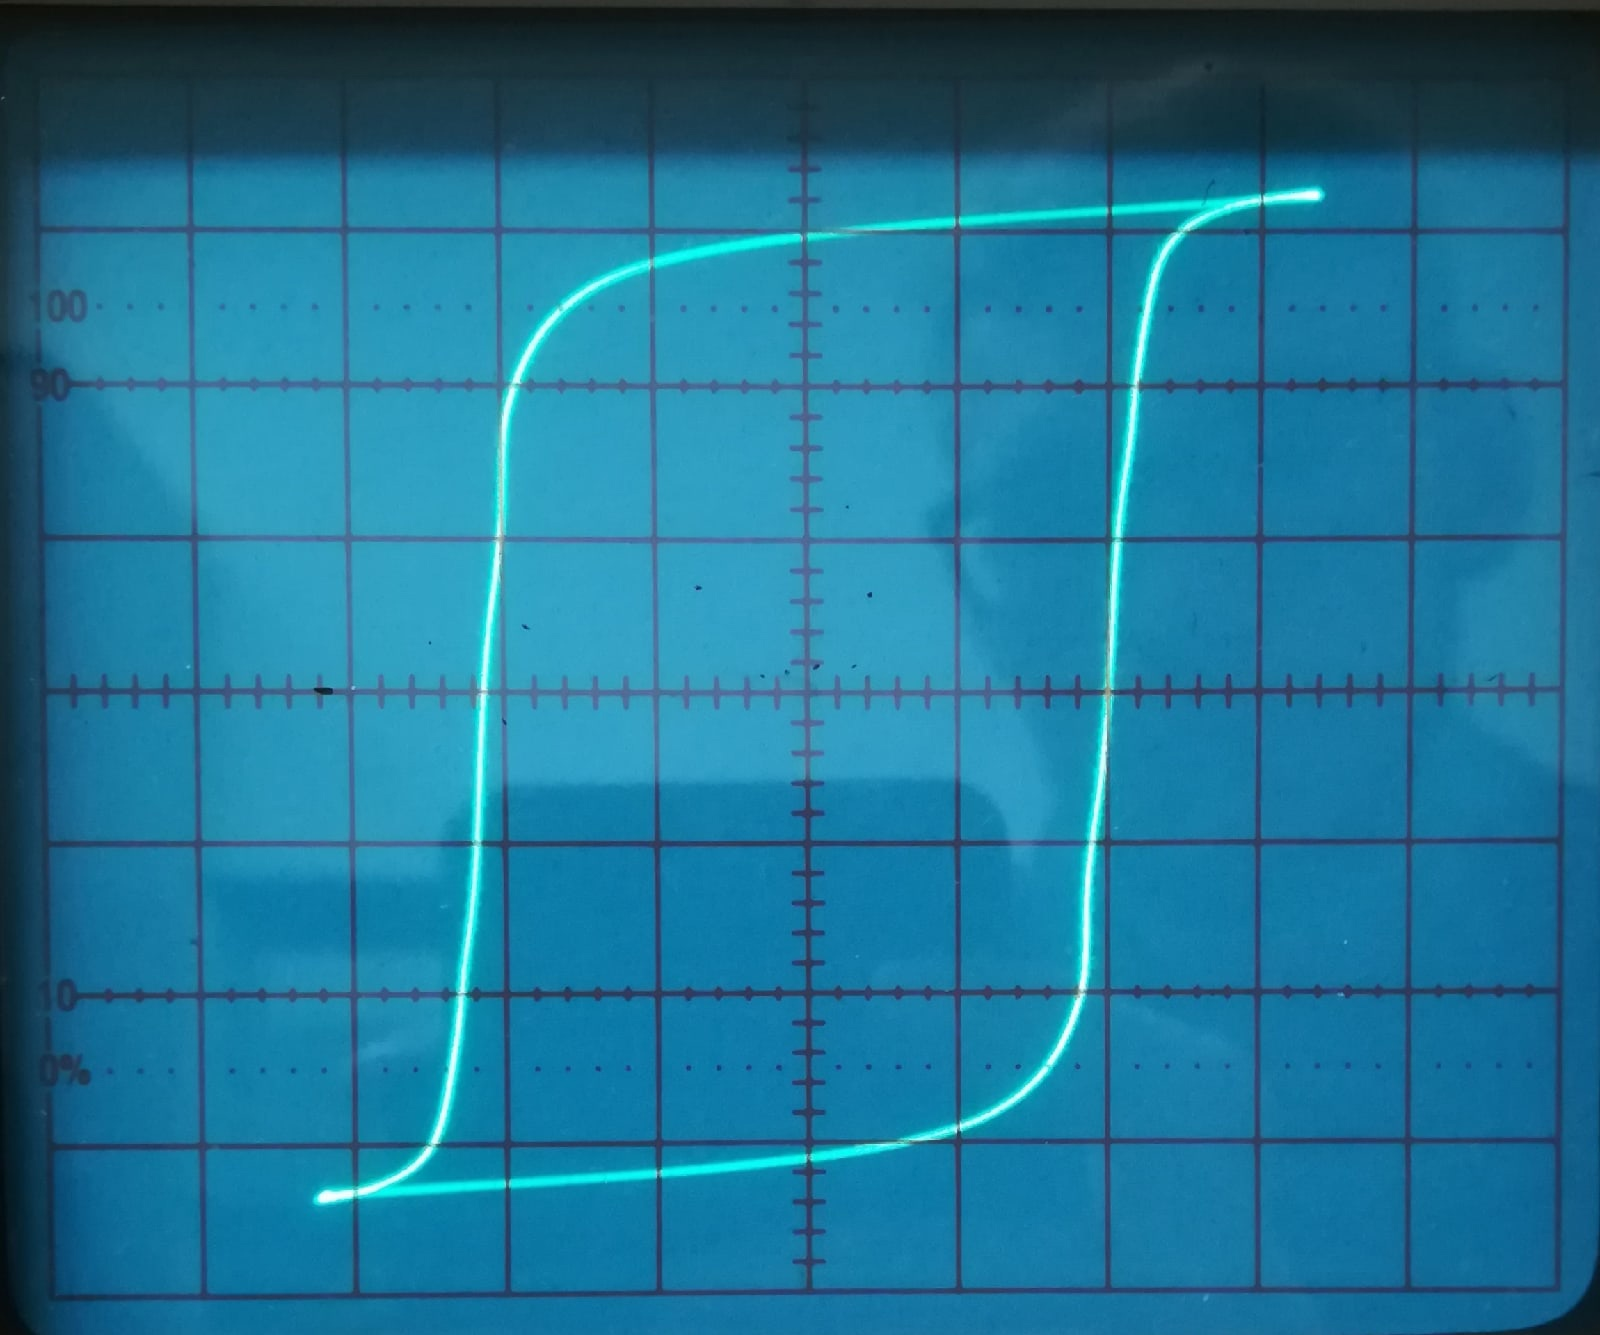
\includegraphics[scale=0.28]{Pictures/ПЕРМАЛЛОЙ_ПЕТЛЯ.jpg}
	\caption{Петля гистерезиса. Пермаллой}
\end{figure}



\newpage
Сведем все данные в таблицу.
\begin{table}[h!]
	\centering
	\begin{tabular}{|l|l|l|l|l|l|l|}
		\hline
		\multicolumn{1}{|c|}{$I_{\text{эф}}$, мА} & \multicolumn{1}{c|}{$I_{\text{эф}} \cdot \sqrt{2}$, мА} & \multicolumn{1}{c|}{$H$, $\frac{\text{А}}{\text{м}}$} & \multicolumn{1}{c|}{$U_{\text{эф}}$, мВ} & \multicolumn{1}{c|}{$U_{\text{эф}} \cdot \sqrt{2}$, мВ} & \multicolumn{1}{c|}{$B$, Тл} & \multicolumn{1}{c|}{$\mu = \dfrac{B}{\mu_0 H}$} \\ \hline
		64,5                                      & 91,217                                                  & 15,20                                                 & 5,2                                      & 7,35                                                    & 0,039                        & 2025,96                                         \\ \hline
		78,3                                      & 110,70                                                  & 18,45                                                 & 10,5                                     & 14,85                                                   & 0,078                        & 3370,75                                         \\ \hline
		87,2                                      & 123,26                                                  & 20,54                                                 & 16,1                                     & 22,77                                                   & 0,120                        & 4641,91                                         \\ \hline
		92,9                                      & 131,38                                                  & 21,90                                                 & 21,4                                     & 30,26                                                   & 0,159                        & 5788,77                                         \\ \hline
		97,6                                      & 138,03                                                  & 23,00                                                 & 27,0                                     & 38,18                                                   & 0,201                        & 6951,88                                         \\ \hline
		101,5                                     & 143,53                                                  & 23,92                                                 & 32,5                                     & 45,96                                                   & 0,242                        & 8047,26                                         \\ \hline
		105,1                                     & 148,63                                                  & 24,77                                                 & 38,0                                     & 53,74                                                   & 0,283                        & 9085,92                                         \\ \hline
		108,2                                     & 153,02                                                  & 25,50                                                 & 43,5                                     & 61,52                                                   & 0,324                        & 10103,00                                        \\ \hline
		111,2                                     & 157,26                                                  & 26,21                                                 & 48,1                                     & 68,02                                                   & 0,358                        & 10870,00                                        \\ \hline
		113,8                                     & 160,90                                                  & 26,82                                                 & 54,5                                     & 77,07                                                   & 0,406                        & 12038,10                                        \\ \hline
		116,2                                     & 164,36                                                  & 27,39                                                 & 60,2                                     & 85,14                                                   & 0,448                        & 13016,80                                        \\ \hline
		118,4                                     & 167,44                                                  & 27,91                                                 & 65,5                                     & 92,63                                                   & 0,488                        & 13902,00                                        \\ \hline
		120,5                                     & 170,41                                                  & 28,40                                                 & 71,0                                     & 100,40                                                  & 0,528                        & 14806,70                                        \\ \hline
		122,8                                     & 173,67                                                  & 28,94                                                 & 76,5                                     & 108,20                                                  & 0,569                        & 15654,90                                        \\ \hline
		125,3                                     & 177,17                                                  & 29,53                                                 & 82,1                                     & 116,10                                                  & 0,611                        & 16468,30                                        \\ \hline
		127,7                                     & 180,54                                                  & 30,09                                                 & 87,4                                     & 123,60                                                  & 0,651                        & 17204,60                                        \\ \hline
		130,8                                     & 184,98                                                  & 30,83                                                 & 93,0                                     & 131,50                                                  & 0,692                        & 17867,50                                        \\ \hline
		133,8                                     & 189,26                                                  & 31,54                                                 & 98,5                                     & 139,30                                                  & 0,733                        & 18495,70                                        \\ \hline
		138,4                                     & 195,73                                                  & 32,62                                                 & 103,9                                    & 146,90                                                  & 0,773                        & 18865,50                                        \\ \hline
		144,7                                     & 204,64                                                  & 34,11                                                 & 109,5                                    & 154,90                                                  & 0,815                        & 19016,60                                        \\ \hline
		154,3                                     & 218,27                                                  & 36,38                                                 & 115,2                                    & 162,90                                                  & 0,857                        & 18756,90                                        \\ \hline
		169,1                                     & 239,14                                                  & 39,86                                                 & 120,6                                    & 170,60                                                  & 0,898                        & 17922,20                                        \\ \hline
		192,3                                     & 271,95                                                  & 45,33                                                 & 126,4                                    & 178,80                                                  & 0,941                        & 16517,90                                        \\ \hline
		216,2                                     & 305,81                                                  & 50,97                                                 & 130,6                                    & 184,70                                                  & 0,972                        & 15177,30                                        \\ \hline
	\end{tabular}
	\caption{Пермаллой}
\end{table}

\newpage
А теперь графики.
\begin{figure}[h!]
	\centering
	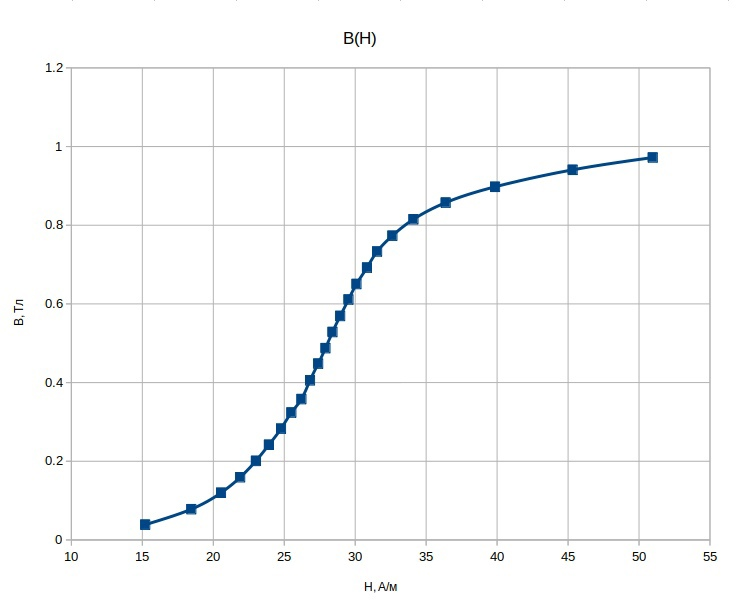
\includegraphics[scale=0.45]{Pictures/ПЕРМАЛЛОЙ_B(H).jpg}
	\caption{Пермаллой. $B(H)$}
\end{figure}

\begin{figure}[h!]
	\centering
	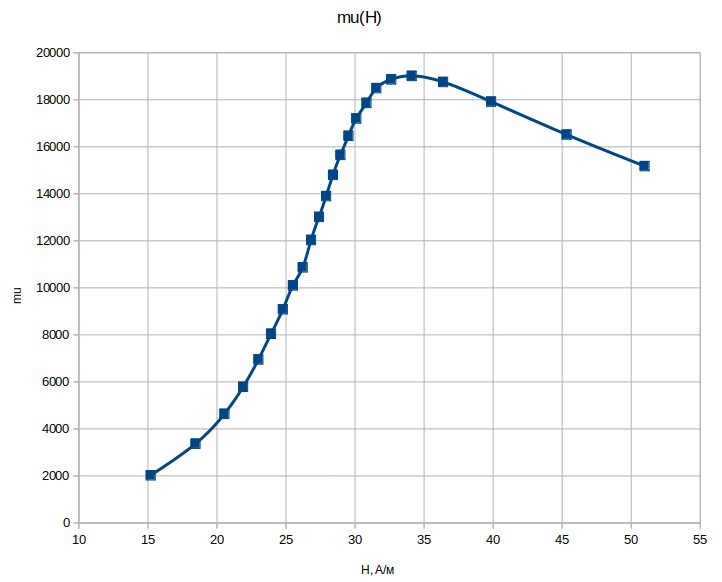
\includegraphics[scale=0.47]{Pictures/ПЕРМАЛЛОЙ_mu(H).jpg}
	\caption{Пермаллой. $\mu (H)$}
\end{figure}



\newpage
\textbf{{\large Кремнистое железо (Fe-Si)}}
\begin{figure}[h!]
	\centering
	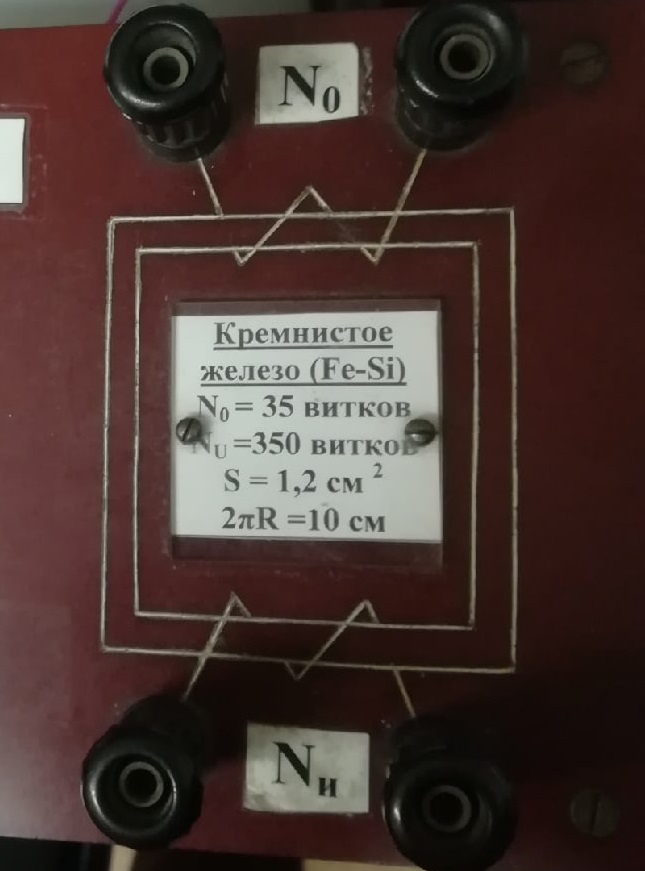
\includegraphics[scale=0.6]{Pictures/КРМЖЛЗ.jpg}
	\caption{Кремнистое железо}
\end{figure}

Параметры образца:

$N_0 = 35;$

$N_u = 350;$

$S = 1,2$ см$^2$;

$2\pi R = 10$ см.

\vspace{7mm}
Предельные значения тока и напряжения:

$I_{\text{пр}} = 877,38$ мА, $U_{\text{пр}} = 167,44$ мВ.
\newpage
\begin{figure}[h!]
	\centering
	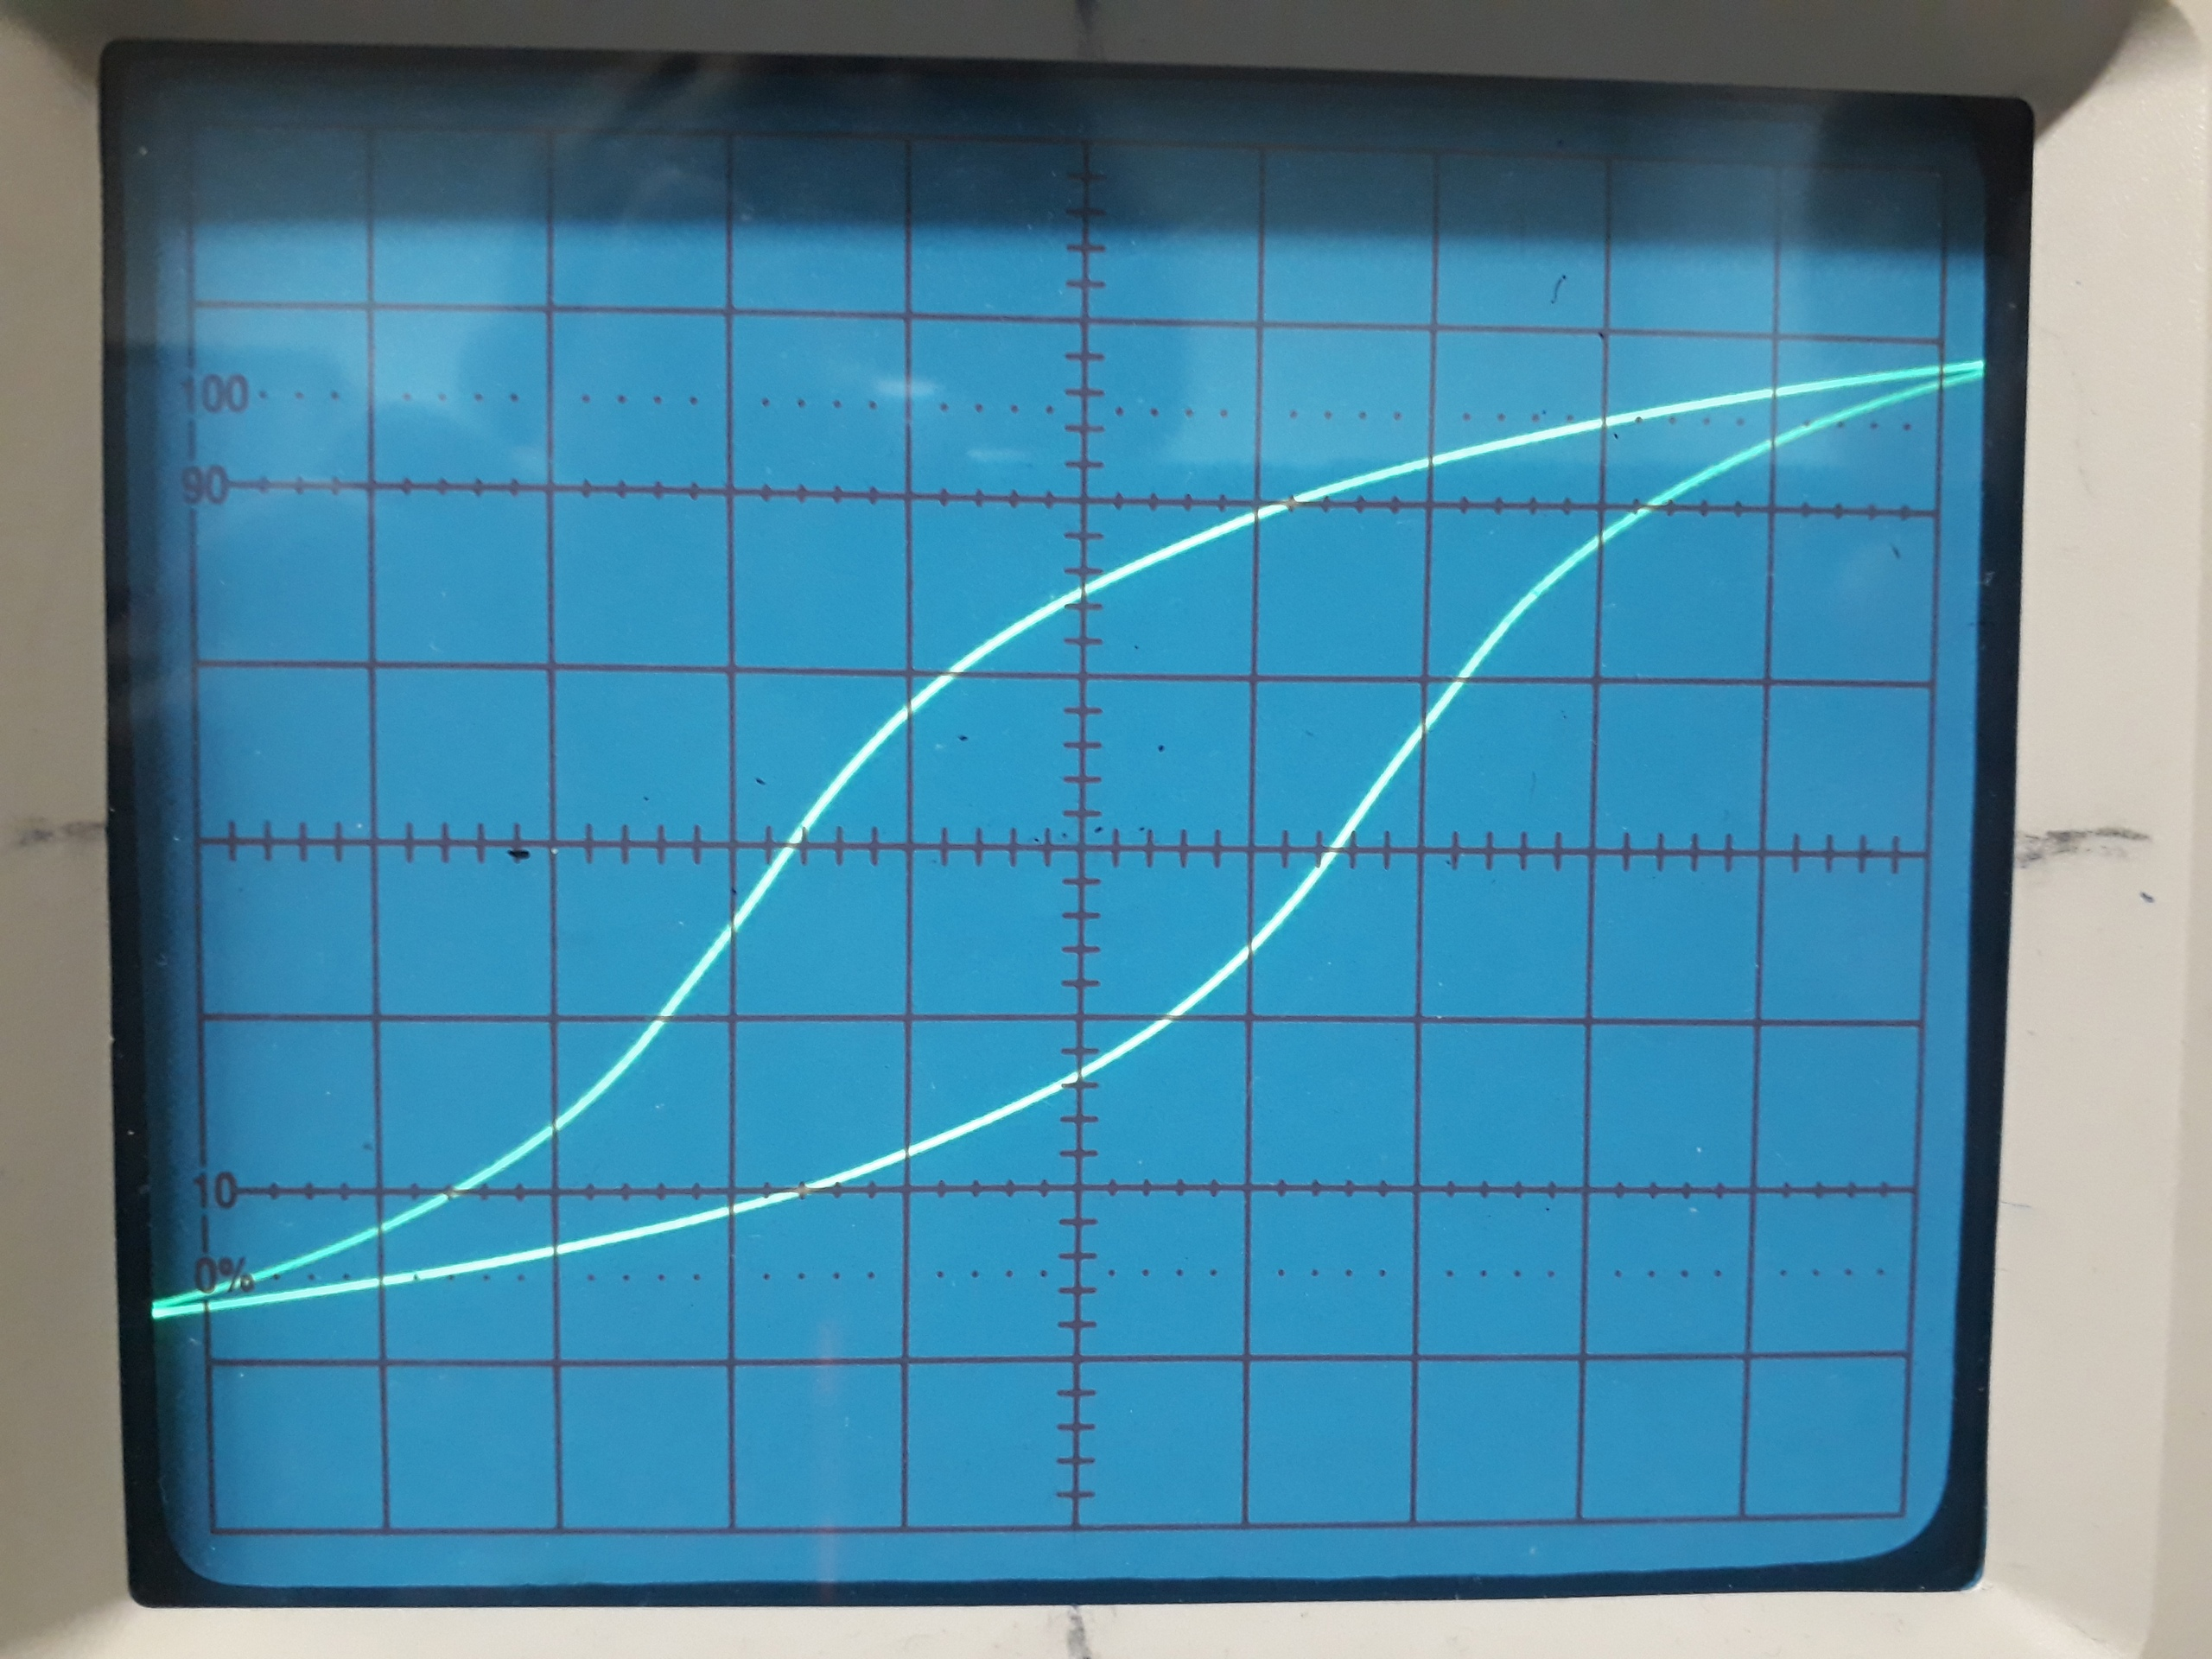
\includegraphics[scale=0.18]{Pictures/КРМЖЛЗ_ПЕТЛЯ.jpg}
	\caption{Петля гистерезиса. Кремнистое железо}
\end{figure}

\end{document}